\fancychapter{Conclusions}
\label{cap:conclusions}

\doublespacing

To wrap up the present thesis, we review the main contributions
developed in this work, and discuss their impact, limitations, and
interesting directions for future work.

\section{Summary of Contributions and Discussion}

\section{Open Problems and Limitations}

\section{Future Directions}

\begin{itemize}
    \item semi-supervision of latent discrete variables and few-shot learning
    \item non-differentiability of the latent discrete variables learning signal
    \item structured latent variables applications in NLP: enumeration can make it easier to learn
\end{itemize}

\section{Broader Impact}

In this chapter, we present the proposed preliminary research ideas
that will be explored in the thesis. In previous works, we explored
how Automatic Post-Editing can improve the quality of NMT with much
less data, how sparse probabilities can aid in interpreting better
the big neural black-box Transformer model, and how these same sparse
probabilities can be used to obtain an efficient method to train
discrete and structured latent variables. Influenced by these works,
we aim to incorporate editing of the target sentence into the NMT
model itself, inspired by APE, and to use structured latent variables
and sparse probabilities to do so. We hypothesize that neural machine
translation might obtain better results by introducing in the system
a mechanism that retrieves translation drafts, which
are edited later on. These drafts might be retrieved in a variety of
ways and from different sources; for example, the drafts might come
from a user-created list of phrase-pairs in the source and target
language, depicting exactly how the user wants some expressions to be
translated. This system will be designed as a deep latent variable
model that aims to disentangle the latent draft creation process from
the encoding of the semantic meaning of the sentence. The model can
be designed in a way such that it is possible to do semi-supervision,
for example, by having an initial phrase table that can be expanded,
or by leveraging monolingual resources. If this proves successful, we
believe this method can obtain great performance in low-resource
machine translation, such as is the case for languages that do not
have a large collection of parallel data, or the case of
domain-specific translations.

Additionally, we propose to create a generative model for
document-level NMT that is inspired by the Neural
Statistician~\citep{edwards2017prociclr}. This work will rely on the
use of a latent structure that summarizes the document in order to
better translate each sentence into the target language.

This proposed work aims to make use of the previous work shown in
previous sections. Automatic Post-Editing, which was discussed in
% \secref{sec:ape_bg} and \secref{cap:ape}, will be useful in designing the
editing component of this NMT system and the transfer learning
techniques discussed in \secref{cap:ape} might prove useful to leverage
monolingual data. In line with the work discussed in
\secref{cap:adaptsparse}, we hope to use sparsity in our models to
improve interpretability of the deep neural model and also to use
sparsity in order to improve efficiency in latent variable training,
as discussed in \secref{cap:sparsemarg}.

% \section{Translating by Editing a Draft}
% \label{sec:draftedits}

\begin{figure}[t]
    \centering
    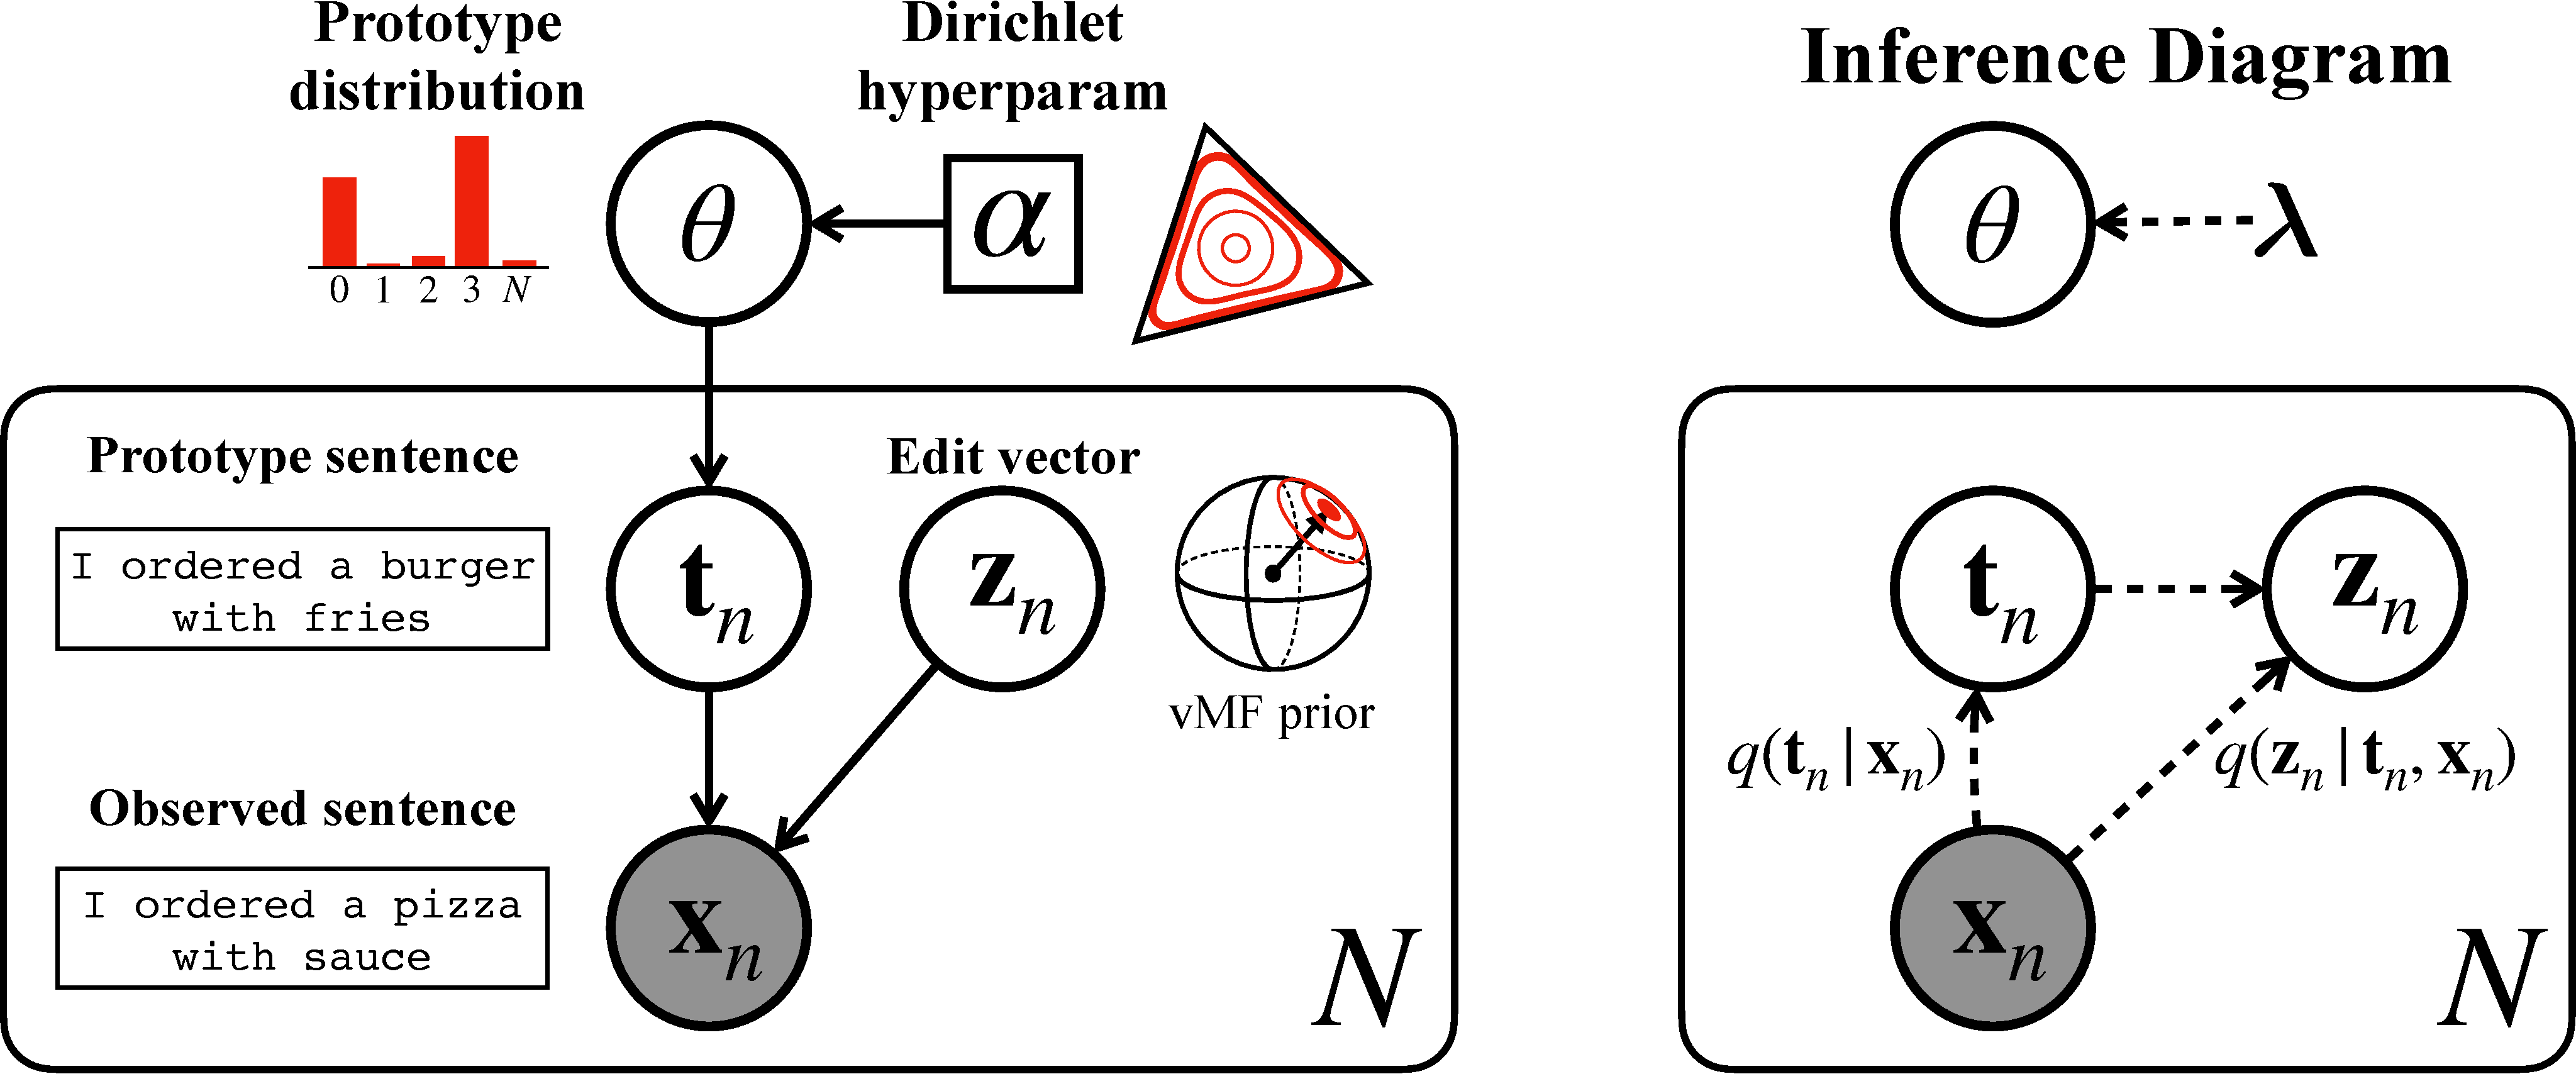
\includegraphics[width=0.8\columnwidth]{heetalmodel.pdf}
    \caption{From \citet{he2020LearningSparsePrototypes}. {\it Left:}
    generative model proposed by
    \citet{he2020LearningSparsePrototypes}. A symmetric Dirichlet
    prior generates $\theta$, a sparse distribution over possible
    prototypes, \ie examples from the training data. In practice, the
    authors choose the entries of $\theta$ that occupy 90\% of the
    probability mass and prune the rest. Then, through SFE, a
    prototype $t$ is chosen from the pruned distribution. From
    editing the chosen prototype, along with information from a
    latent continuous edit vector $z$ with a vMF
    prior~\citep{s-vae18}, the final sentence
    $x$ is produced. {\it Right:} inference model. The edit
    vector is inferred from the prototype and $x$, while the
    prototype retriever is only inferred from $x$.
    \label{fig:he2020LearningSparsePrototypes}}
\end{figure}

The proposed NMT model in this section is based on previously
published work on prototype editing for language
modeling~\citep{guu2018GeneratingSentencesEditing,
    he2020LearningSparsePrototypes}. In this generative model, the
generative process has two main steps: (1) selecting a prototype
$\bm{t}$ from a list of possible prototypes (\eg the training data),
and (2) editing that prototype by sampling an edit vector $\bm{z}$
that encodes the type of edit (\eg active to passive, reordering,
etc.) and generate a new sentence $\bm{x}$ by editing $\bm{t}$
according to $\bm{z}$. The language model described then factorizes
as

\begin{equation}
    p(\bm{x}) = \sum_{\bm{t} \in \mathcal{X}} p(\bm{x} | \bm{t}) p(\bm{t}),
\end{equation}

\noindent where $\mathcal{X}$ is the training data of the model.
Consequently, in practice, this model requires for the whole training
data $\mathcal{X}$ to be searched over in order to retrieve a
prototype.

Recently, \citet{he2020LearningSparsePrototypes} proposed an
improvement on this system in which prototypes are sampled from a
latent distribution, which in turn is sampled from a Dirichlet prior
(\figref{fig:he2020LearningSparsePrototypes}). This choice of prior
allows for a sparse selection of prototypes, improving the efficiency
of the model during prototype retrieval from the training data.

Under this model, the data has the following log marginal likelihood:

\begin{equation}
    \log p(\bm{X} ; \gamma, \alpha) =
    \log \int_\theta p_\alpha (\theta)
    \left[ \prod_n \sum_{t} \int_{z}
        p(t | \theta) p(z) p(x | t, z)
        dz \right] d\theta
\end{equation}

In this model, $p_\alpha(\theta)$ is the prior over the prototype
distribution, $p(z)$ is the prior over the edit vector, and
$p(z) p(x | t, z)$ is {\it the editor}.
The prior over prototypes is a Dirichlet parameterized by $\alpha$,
which outputs a projection onto the $N-1$ simplex, with a preference
for ``sparse'' solutions when $\alpha<1$. Following
\citet{guu2018GeneratingSentencesEditing} the prior over the edit
vector $z$ is the von-Mises Fisher (vMF)
distribution~\citep{s-vae18}. Finally, the editor
$p(z) p(x | t, z)$ is a
sequence-to-sequence model from $t$ to $x$ with
$z$ incorporated. Learning is achieved by optimizing the ELBO,
with inference done as depicted in
\figref{fig:he2020LearningSparsePrototypes} on the right side.

\begin{figure}[t]
    \centering

    \begin{tikzpicture}
        % Define nodes
        \node[obs]                (y)     {$ y $};
        %\node[semi, left =of y]   (x) {$ x $};
        \node[latent, above =of y] (t) {$ t $};
        \node[latent, left =of t] (z) {$ z $};
        \node[obs,below =of z]   (x) {$ x $};

        % Connect nodes
        \edge{x}{z,t};
        \edge{t,z}{y};

        \plate{data}{(x)(y)(t)(z)}{$N$};
    \end{tikzpicture}
    ~
    \begin{tikzpicture}
        % Define nodes
        \node[obs]                (y)     {$ y $};
        %\node[semi, left =of y]   (x) {$ x $};
        \node[latent, above =of y] (t) {$ t $};
        \node[latent, left =of t] (z) {$ z $};
        \node[obs,below =of z]   (x) {$ x $};

        % Connect nodes
        \edge[dashed]{y}{z};
        \edge[dashed]{y}{t};

        \plate{data}{(x)(y)(t)(z)}{$N$};
    \end{tikzpicture}

    \caption{Generative model (left): $z$ and $t$ are modelled
        conditioned on $x$, $y$ is independent of $x$ given $z$ and $t$.
        Inference model (right): we ignore $x$ and model $z$ and $t$
        independently given $y$.} \label{fig:conditional}
\end{figure}

While \citet{he2020LearningSparsePrototypes} apply their sparse neural editor
to language modelling, we will model instead a conditional
distribution over $\mathcal{X} \times \mathcal{Y}$, i.e. a
machine translation model. We propose to model this distribution
as the marginal of a deep latent variable model
\begin{align}
    p(y, t, z|x, \theta) & =
    p(t | x, \theta)p(z |x, \theta)p(y |t, z, \theta)
\end{align}

\noindent where $t$ is a discrete/structured latent variable and $z$ is a
continuous representation. See \figref{fig:conditional} (left).
Instead of $t$ being a pointer to a sentence in the training data, we
think of $t$ as being a template for $y$---it can be a lexicalised
rule with gaps/variables, phrase-based mapping from $x$ to a string
in the target language, etc.
% While the nature of $t$ is not yet
% defined in the scope of this thesis, we will exemplify the latter
% option in \secref{sec:transduction}.

We can express a lowerbound on the logarithm of the conditional likelihood for an observation $(x,y)$,
\begin{align}
    \log p(y|x, \theta) & \ge \mathbb E_{q(z,t|y,\lambda)}\left[ \log p(y|z,t, \theta) \right] \nonumber                                \\
                        & - \KL(q(z, t|y,\lambda) || p(z, t|x, \theta))                                                                 \\
                        & \overset{\text{MF}}{=} \mathbb E_{q(z|y,\lambda)q(t|y,\lambda)}\left[ \log p(y|z,t, \theta) \right] \nonumber \\
                        & - \KL(q(z|y,\lambda) || p(z|x,\theta)) - \KL(q(t|y,\lambda) || p(t|x, \theta)) ~.
\end{align}

For better disentanglement it's also useful to use constraints that
promote low mutual information $I(Z;T|X)$: note that though we design
the generative components to be independent, we train an
approximation to the true posterior, which may lead to correlated $z$
and $t$ for any given $x$. For example,
\citet{chengImprovingDisentangledText2020} use a mutual information
objective in order to disentangle latent variables in text
generation. In essence, they {\bf minimize} the mutual information
between two different latent variables---one related to the semantic
content, $c$, and another to the style, $s$---while maximizing the
mutual information between $x$ and $c$, and between $y$ and $s$.

\paragraph*{Caveats} Note that because of the conditional formulation,
this model lacks constraints on $z$ and $t$, in other words,
$p(z,t|x,\theta)$ is controlled by a NN and is only constrained by
the choice of parametric family we employ. It may be necessary to
impose some form of marginal constraints on $\mathbb
    E_X[p(z|x,\theta)]$ and $\mathbb E_X[p(t|x,\theta)]$. Another caveat
is conceptual: our graphical model establishes conditional
independence $Z \perp T | X$, whereas disentangled representations
should be \emph{marginally independent}.

% \subsection{\label{sec:transduction}Translation by Transducing}

Suppose we have a grammar $\mathcal T$ that allows us to identify a
set $\mathcal T(x)$ of \emph{derivations}, each of which maps $x$ to
some sentence in the target language. A derivation $t \in \mathcal
    T(x)$ is a sequence of operations that rewrite $x$ into a sentence in
the target language. In this section we describe a component $p(t|x,
    \theta, \mathcal T)$, a probability distribution over the derivations
supported by a grammar that corresponds to a phrase-based transducer.
The key to this component is an efficient representation of the set
$\mathcal T(x)$: a directed acyclic graph whose size is a polynomial
function of sentence length. Once this representation is in place, we
score its arcs independently using NNs. Let us assume that a
derivation $t$ is represented by a sequence of $|t|$ arcs and $t_i$
is the $i$th arc in the derivation. The probability of a derivation
$t$ given a source sentence $x$ is given by

\begin{align}
    p(t|x, \theta) =
    \frac
    {\exp(\sum_{i=1}^{|t|} f(x, t_i, \theta))}
    {\sum_{t' \in \mathcal T(x)}
        \exp(\sum_{i=1}^{|t'|} f(x, t'_i, \theta))
    }
\end{align}

\noindent which is a Gibbs distribution whose support is $\mathcal
    T(x)$. We use an efficient parameterisation based on arc potentials,
though note that \emph{efficiency} here really depends on the size of
the sample space of arcs. Note that the denominator sums over the
space of all possible derivations compatible with $x$, a computation
that scales linearly in the size of the graph that represents
$\mathcal T(x)$---this is done via the forward
algorithm.\footnote{Because our Gibbs is built on a DAG and we will
    keep this DAG polynomial in size, every algorithm in the book is
    available: forward, Viterbi, ancestral sampling.} Later, we
will aim at a sparse alternative to the Gibbs distribution, that is,
with support in a small subset of $\mathcal T(x)$.

% \section{NMT through Latent Summary}

\begin{figure}[t]
    \centering
    \begin{tikzpicture}
        % Define nodes
        \node[obs]                (y)     {$ y $};
        \node[obs, left =of y]   (xi) {$ X $};
        \node[latent, above =of xi] (z) {$ z $};

        % Connect nodes
        \edge{xi,z}{y};
        \edge{xi}{z};

        \plate{data}{(y)}{$N$};
    \end{tikzpicture}
    ~
    \begin{tikzpicture}
        % Define nodes
        \node[obs]                (y)     {$ y $};
        \node[obs, right =of y]   (xi) {$ X $};
        \node[latent, above =of xi] (z) {$ z $};

        % Connect nodes
        \edge[dashed]{xi,y}{z};

        \plate{data}{(y)}{$N$};
    \end{tikzpicture}

    \caption{{\it Left}: a simple generative model for document-level
        NMT with interesting properties. Given $z$, there is full
        independence between $y_i$, but at test time there is an implicit
        dependency.
            {\it Right}: inference model. $X$ and $y_i$ infer $z$.}
    \label{fig:doclevel}
\end{figure}

In this section, we build upon the generative model designed in
\citet{edwards2017prociclr}. In that work, the authors use a {\it
        neural statistician}---a generative model that gets a dataset as
input and is able to construct a continuous latent summary $c$ of
that dataset, which in turn allows the model to get better latent
representations $z$ for unsupervised and few-shot learning.

To extend this idea to NMT, we consider $c$ to be a structured latent
variable (instead of a continous one), which selects the sentences of
a document that best describe it. An interesting consequence of using
a structured latent variable in this application is the ability to
use a budget factor to constrain the number of sentences selected. We
hypothesize that this idea could be tested in two applications:
multi-domain NMT and document-level NMT.

% \subsection{Multi-domain Learning}

Here $c$ will be a summary of the current domain to be translated,
and will help $z$ to encode any topic specific content that a NMT
model could have trouble to translate without the proper context.
Another possibility for $c$ is for this latent variable to be a
choice of words over the vocabulary.

A possible model is depicted in \figref{fig:indomainstatistician}.

\begin{figure}[t]
    \centering
    \begin{tikzpicture}
        % Define nodes
        \node[obs]                (x)     {$ x $};
        \node[obs, below =of x]   (y) {$ y $};
        \node[latent, right =of y] (z) {$ z $};
        \node[latent, above =of x, xshift=1.75cm] (c) {$ c $};

        % Connect nodes
        \edge{x,z}{y};
        \edge{c}{z};
        \edge{x}{c};

        \plate{data}{(y)(x)(z)}{$N$};
    \end{tikzpicture}
    ~
    \begin{tikzpicture}
        % Define nodes
        \node[obs]                (x)     {$ x $};
        \node[obs, below =of x]   (y) {$ y $};
        \node[latent, right =of y] (z) {$ z $};
        \node[latent, above =of x, xshift=1.75cm] (c) {$ c $};

        % Connect nodes
        \edge[dashed]{y}{z};
        \edge[dashed]{x,y}{c};

        \plate{data}{(x)(y)(z)}{$N$};
    \end{tikzpicture}

    \caption{{\it Left}: each sentence $x_i$ is translated to $y_i$
        while $c$ and $z$ encode in-domain specific representations; $c$
        encodes the summary of the in-domain dataset and $z$ the
        translation representation of this summary into the target
        language.
            {\it Right}: inference model. $y_i$ infers $z$ and the whole
        in-domain document $X$ infers $c$.}
    \label{fig:indomainstatistician}
\end{figure}

% \subsection{Document-level NMT}

In document-level NMT, a document with $M$ sentences $X=[x_1, \dots,
    x_M]$ in the source language is translated to a target language and
forms a document with $N$ sentences $Y=[y_1, \dots, y_N]$. In the
model depicted in \figref{fig:doclevel}, the sentences in the
document $Y$ are only independent of each other given $z$, thus
having an implicit dependency between the sentences that is encoded
within $z$. This model can potentially mitigate posterior
collapse~\footnote{Posterior collapse is a common issue in
    variational models with powerful decoders. Due to the auto-regressive
    nature of most sequence neural models, the decoder tends to ignore
    the approximated posterior computed by the encoder and, consequently,
    a useful posterior is not learned.} since the model needs to use $z$
in order to get document-level information. This property also
provides the model good memory footprint.

A model with latent summary is shown in
\figref{fig:doclevelstatistician}. This is an evolved model of the
one described above, now including a latent summary $c$. In this
case, contrasting with the model example in
\figref{fig:indomainstatistician}, the summary is created through the
target document.
% A possible way to do this connects with
% \secref{sec:draftedits}, where there could be a memory of phrases
% used to encode $c$ (see \secref{sec:transduction}) that are used for
% agreement in documents of the target language.

\begin{figure}[t]
    \centering
    \begin{tikzpicture}
        % Define nodes
        \node[obs]                (y)     {$ y $};
        \node[latent, above =of y] (z) {$ z $};
        \node[latent, left =of z] (c) {$ c $};
        \node[obs, left =of y]   (xi) {$ X $};

        % Connect nodes
        \edge{xi,z}{y};
        \edge{c}{z};
        \edge{xi}{c};

        \plate{data}{(y)(z)}{$N$};
    \end{tikzpicture}
    ~
    \begin{tikzpicture}
        % Define nodes
        \node[obs]                (y)     {$ y $};
        \node[latent, above =of y] (z) {$ z $};
        \node[latent, right =of z] (c) {$ c $};
        \node[obs, right =of y]   (xi) {$ X $};

        % Connect nodes
        \edge[dashed]{y}{z};
        \edge[dashed]{y,xi}{c};

        \plate{data}{(y)(z)}{$N$};
    \end{tikzpicture}

    \caption{{\it Left}: document-level NMT with a latent summary.
        The latent $c$ encodes a summary representation of the document.
        This summary is then used to encode
        document-level features into $z$. Then each $y_i$ is translated
        independently given the source document and $z$. {\it Right}:
        inference model. $y_i$ infers $z$ and the whole in-domain
        document $Y$ infers $c$.}
    \label{fig:doclevelstatistician}

\end{figure}

\cleardoublepage

\singlespacing